
%%%%%%%%%%%%%%%%%%%%%%%%%%%%%%%%%%%%%%%%%%%%%%%%%%%%%%%%%%%%%%%
%
% Welcome to Overleaf --- just edit your LaTeX on the left,
% and we'll compile it for you on the right. If you open the
% 'Share' menu, you can invite other users to edit at the same
% time. See www.overleaf.com/learn for more info. Enjoy!
%
%%%%%%%%%%%%%%%%%%%%%%%%%%%%%%%%%%%%%%%%%%%%%%%%%%%%%%%%%%%%%%%
\documentclass{beamer}
\usepackage{braket}
\usepackage{amsmath}

%Information to be included in the title page:
\title{HHL - Algorithmus}
\author{Alfred Nguyen}
\institute{Fakultät der Informatik \\
Technische Universität München \\
  85758 Garching, Bavaria
}
\date{June 2023}

\setbeamertemplate{navigation symbols}{}
\setbeamertemplate{footline}[frame number]

\AtBeginSection[]
{
  \begin{frame}
    \frametitle{Gliederung}
    \tableofcontents[currentsection]
  \end{frame}
}

\begin{document}

  \frame{\titlepage}
  \begin{frame}
    \frametitle{Gliederung}
    \tableofcontents
  \end{frame}
  
%\section{Einführung}

%\subsubsection{Quanten Algorithmen}

    \begin{frame}
        \frametitle{Einführung}
        Wir haben schon viel über die wichtigsten Algorithmen gehört
        \begin{itemize} 
            \item  Shors-Algorithmus
            \item  Grover-Algorithmus
        \end{itemize}

        \hfill

\onslide<2>{
        Der HHL-Algorithmus
        \begin{itemize}
            \item  erstellt von Aram Harrow, Avinatan Hassidim und Seth Lloyd 
            \item  lösen von sehr großen linearen Gleichungen 
        \end{itemize}

        $$ A \vec{x} = \vec{b} $$
}

    \end{frame}


%\subsubsection{Motivation}

    \begin{frame}
        \frametitle{Motivation}

        Es löst grundlegendes Probleme in der Mathematik
        \begin{itemize}
            \item   Least square fitting 
            \item   Optimierungs Probleme
            \item   Simulationen und Imageprocessing
            \item   ...
       \end{itemize}

        \hfil

    \end{frame}

%\subsubsection{Das Problem}
    \begin{frame}
        \frametitle{Das Problem}


        \textbf{Gegeben:}
        \begin{itemize}
            \item Matrix $A$ der Form $n \times n$
            \item Vektor $\vec{b}$
       \end{itemize}

       \hfill

\onslide<2,3>{
       \textbf{Löse das System:}
        $$A \vec{x} = \vec{b}$$

        $$\vec{x} = A^{-1} \vec{b}$$
}
       \hfill

\onslide<3>{

        Wir sind also daran interessiert das Inverse $A^{-1}$ zu finden
}

    \end{frame}
        

%\section{Mathematische Grundlagen}

\begin{frame}
    \frametitle{Hermitsche Matrix}
    \textbf{Sei: }
    \begin{itemize}
        \item   $A$ eine $n \times n$ Matrix
        \item   $A^T$ das transponierte von $A$
        \item   $\overline A$  das komplex konjugierter von $A$
        \item   $A^\dagger$ die Hermitsche Matrix von A
   \end{itemize}

   \hfil

    \textbf{Dann:}
    $$A = \overline {A^T} = A^\dagger $$
\end{frame}

\begin{frame}
    \frametitle{Hermitsche Matrix}
    
    \textbf{Beispiel:}
    $$A=\begin{bmatrix}2 & 1-i \\ 1+i & 3 \\ \end{bmatrix}$$
    $$\overline A = \begin{bmatrix} 2 & 1+i \\ 1-i & 3 \end{bmatrix}$$
    $$\overline {A^T} = \begin{bmatrix} 2 & 1-i \\ 1+i & 3 \\ \end{bmatrix}= A = A^\dagger$$

    \hfil

    \hfil

    Die Matrix $A$ ist Hermitisch.
\end{frame}

\begin{frame}
    \frametitle{Hermitsche Matrix}
    
    Falls eines Matrix $A$ nicht Hermitisch ist:

    \hfil

    $$A^\dagger = \begin{pmatrix} 0 & A \\ \overline {A^T} & 0 \end{pmatrix}$$
\end{frame}


\begin{frame}
    \frametitle{Spektralzerlegung}

    \textbf{Gegeben: }

    $$A =  U D U^T$$

    $$= \begin{bmatrix} U_1&U_2&...&U_n \end{bmatrix}
    \begin{bmatrix} \lambda_1 & 0 & 0 & 0\\ 0 & \lambda_2 &0 & 0\\ 0 & 0 & ... & 0\\ 0 & 0 & 0& \lambda_n \\ \end{bmatrix}
    \begin{bmatrix} U_1\\ U_2\\ ...\\ U_n\end{bmatrix}$$

    \hfil

    \begin{itemize}
        \item   $A$ eine $n \times n$ Matrix
        \item   $D$ ist eine Diagonalmatrix aus den Eigenwerten
        \item   $U$ besteht aus den Eigenvektoren von A
   \end{itemize}



    \hfil

    $A$ lässt sich aus seinen Eigenweren und Eigenvektoren darstellen.

\end{frame}

\begin{frame}
    \frametitle{Spektralzerlegung}
    Selbes gilt für das Inverse von $A$ 

    $$A^{-1}=  U^T D^{-1} U$$

    \hfil

    \begin{itemize}
        \item  $A^{-1}$ nur durch Eigenwerten und Eigenvektoren bestimmbar!
        \item  Methode im klassischen nicht schneller
        \item  für HHL Algorithmus sehr wichtig
   \end{itemize}
\end{frame}

\begin{frame}
    \frametitle{Veschränkung}
    
    Verschränkte Zustände können nicht durch einzelne Zustände dargestellt werden

    \hfil

    $$\ket{\Phi} \neq \ket{\phi} \ket{\psi}$$

\end{frame}

\begin{frame}
    \frametitle{Veschränkung}
    \textbf{Beispiel:}

    \hfil

    \begin{columns}[c]
        \begin{column}{0.6\hsize}\centering
        Nicht Verschränkt
        $$\ket{\Phi_1} = \frac{1}{\sqrt{2}} ( \ket{10} + \ket{11})$$
        $$= \ket{1}\otimes \frac{1}{\sqrt{2}} ( \ket{0} + \ket{1})= \ket{1} \ket{+}$$
        \end{column}

        \begin{column}{0.4\hsize}
        Verschränkt
        $$\ket{\Phi_2} = \frac{1}{\sqrt{2}} ( \ket{00} + \ket{11})$$
        $$\neq \ket{\alpha}\ket{\beta}$$

        \end{column}
    \end{columns}

\end{frame}
%\section{HHL Algorithmus}

%\subsubsection{Übersicht}

    \begin{frame}
    \frametitle{Übersicht}
    Vergleich klassische zur quanten Version

    \hfil

    \begin{columns}[c]
        \begin{column}{0.6\hsize}\centering
        Klassisch
        $$A \vec{x} = \vec{b}$$
        $$\vec{x} = A^{-1}\vec{b}$$
        \end{column}

        \begin{column}{0.4\hsize}
        Quanten Version
        $$A \ket{x} = \ket{b}$$
        $$\ket{x} = A^{-1}\ket{b}$$
        \end{column}
    \end{columns}

    \hfil

    \hfil
    
    Spektralzerlegung von $A$ und $\ket{b}$
    $$\ket{x} =  A^{-1} \ket{b} = \sum_{i=0}^{2^{n_b}-1} \lambda_i^{-1} b_j\ket{u_j}$$

    \end{frame}


%\subsubsection{Der Algorithmus}

    \begin{frame}
    \frametitle{Der Algorithmus}

        \textbf{Ablauf}
        \begin{enumerate}
            \item State Preparation
            \begin{itemize}
                \item Enkodiert Vektor und Matrix in Quanten Computer
            \end{itemize}
            \item Quantum Phase Estimation
            \begin{itemize}
                \item ermittelt Eigenwerte 
            \end{itemize}
            \item Ancilla Bit Rotation 
            \begin{itemize}
                \item  Invertiert Eigenwerte
            \end{itemize}
            \item Inverse Quantum Phase Estimation
             \begin{itemize}
                \item löst verschränkte Qubits auf
            \end{itemize}
            
            \item Messung
             \begin{itemize}
                \item liest das Ergebnis $\ket{x}$ aus
            \end{itemize}
 
        \end{enumerate}

    \end{frame}

\begin{frame}
    \frametitle{Quantum Circuit}
    \begin{center}
    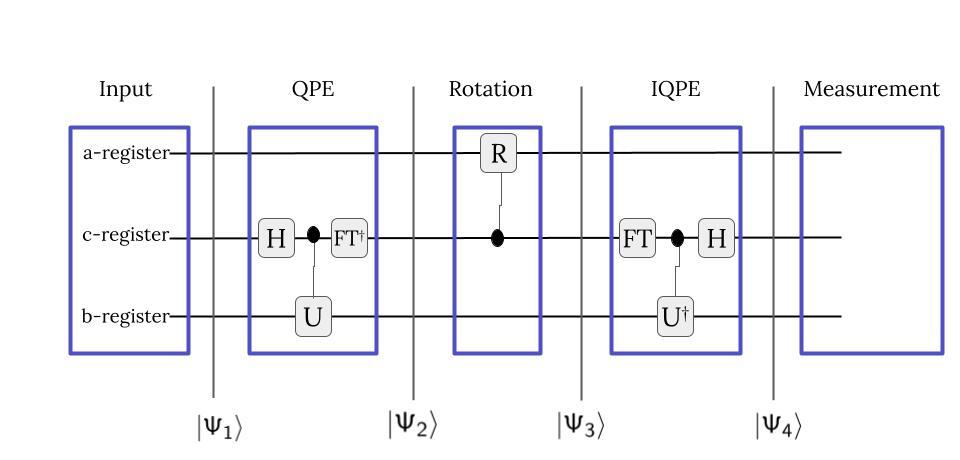
\includegraphics[width=10.5cm]{img/hhl_circuit/hhl_circuit.jpg}
    \end{center}
    \begin{enumerate}
        \item Ancilla (Helfer): a-register
        \begin{itemize}
            \item Indikator qubit, zeigt ob Zustände verschränkt sind
        \end{itemize}

        \item Register: c-register
        \begin{itemize}
            \item beinhaltet die Eigenwerte
        \end{itemize}
        
        \item Input: b-register 
        \begin{itemize}
            \item beinhaltet den Vektor $\vec{b}$
        \end{itemize}
        
    \end{enumerate}
   \end{frame}

%\section{Einfaches Beispiel}

\begin{frame}
    \frametitle{Einfaches Beispiel}

    Matrix $A$ und Vektor $\vec{b}$:
    \begin{columns}[c]
        \begin{column}{0.5\hsize}\centering
            $$A = \begin{pmatrix} 1 & -\frac{1}{3}\\ -\frac{1}{3} & 1\\ \end{pmatrix}$$
        \end{column}

        \begin{column}{0.5\hsize}
            $$\vec{b} = \begin{pmatrix} 0 \\ 1\\ \end{pmatrix}$$
        \end{column}
    \end{columns}
 
    \hfil

    \hfil

\onslide<2>{
    Klassische Lösung
    \begin{columns}[c]
        \begin{column}{0.5\hsize}
            \centering
            $$\vec{x} = \begin{pmatrix} \frac{3}{8}\\ \frac{9}{8}\\ \end{pmatrix}$$
        \end{column}

        \begin{column}{0.5\hsize}
            \centering
            Verhältnis der Lösung:
            $$\frac{ |x_0|^2}{ |x_1|^2}= \frac{\frac{9}{64}}{\frac{81}{64}} = \frac{1}{9}$$
        \end{column}
    \end{columns}
 }


\end{frame}

\begin{frame}
    \frametitle{Einfach Beispiel}


    Eigenvektoren von $A$ sind:    
    \begin{columns}[c]
        \begin{column}{0.5\hsize}\centering
            $$ \vec{u_0} = \begin{pmatrix} \frac{-1}{\sqrt{2}}\\ \frac{-1}{\sqrt{2}}\\ \end{pmatrix}$$
        \end{column}
        \begin{column}{0.5\hsize}
            $$\vec{u_1} = \begin{pmatrix} \frac{-1}{\sqrt{2}}\\ \frac{1}{\sqrt{2}}\\ \end{pmatrix}$$
        \end{column}
    \end{columns}

    \hfil

    \hfil

\onslide<2>{
    Enkodiert
    \begin{columns}[c]
            \begin{column}{0.5\hsize}\centering
                $$ \ket{u_0} = \frac{-1}{\sqrt{2}}\ket{0} + \frac{-1}{\sqrt{2}}\ket{1}$$
            \end{column}
            \begin{column}{0.5\hsize}
                $$\ket{u_1}= \frac{-1}{\sqrt{2}}\ket{0} + \frac{1}{\sqrt{2}}\ket{1}$$
            \end{column}
        \end{columns}

}
\end{frame}

\begin{frame}
    \frametitle{Einfach Beispiel}

    Eigenvektoren von $A$ sind:    
    \begin{columns}[c]
        \begin{column}{0.5\hsize}\centering
            $$\lambda_0 = \frac{2}{3}$$
        \end{column}

        \begin{column}{0.5\hsize}
            $$\lambda_1 = \frac{4}{3}$$
        \end{column}
    \end{columns}

    \hfil

    \hfil

\onslide<2>{
    Einkodiert:
    \begin{columns}[c]
        \begin{column}{0.5\hsize}\centering
            $$\ket{\widetilde{\lambda_0}} = \ket{01}$$
        \end{column}

        \begin{column}{0.5\hsize}
            $$\ket{\widetilde{\lambda_1}} = \ket{10}$$
        \end{column}
    \end{columns}
}
\end{frame}




\begin{frame}
    \frametitle{Ablauf}

    \begin{center}
    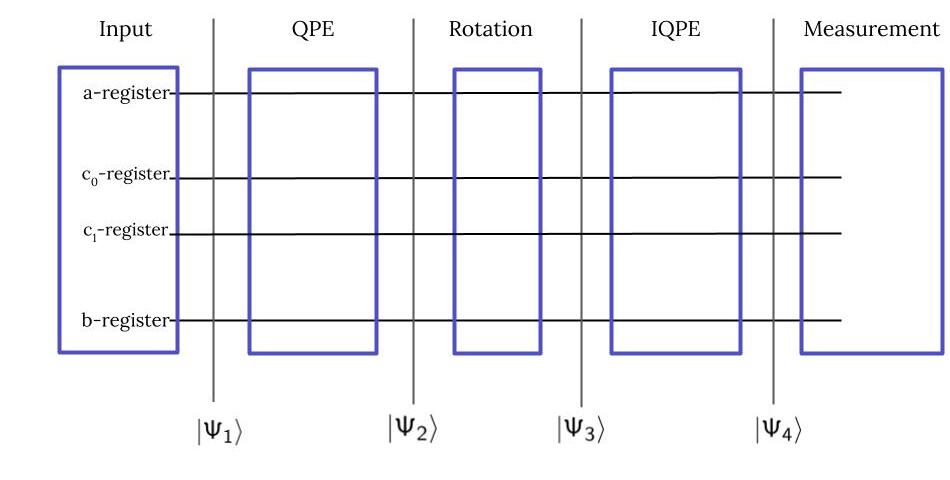
\includegraphics[width=10.5cm]{img/example_circuit/example_circuit.jpg}
    \end{center}

    \begin{enumerate}
        \item Anzahl Qubit for a-register: 1
        \item Anzahl Qubits für das c-Register: N = 2
        \item Anzahl Qubits für $\vec{b}$: $n_b = log_2(N) = log_2 (2) = 1$ 
    \end{enumerate}
\end{frame}

\begin{frame}
    \frametitle{State Preparation}

    \begin{itemize}
        \item $\vec{b}$ wird als Quantenzustand $\ket{b}$ kodiert
        \item in unserem Fall ist es sehr einfach
    \end{itemize}

    $$\vec{b} = \begin{pmatrix} 0\\ 1\\ \end{pmatrix} \Leftrightarrow \ket{b} = 0 \ket{0} + 1 \ket{1} = \ket{1}$$
\end{frame}


\begin{frame}
    \frametitle{State Preparation}

    \begin{center}
    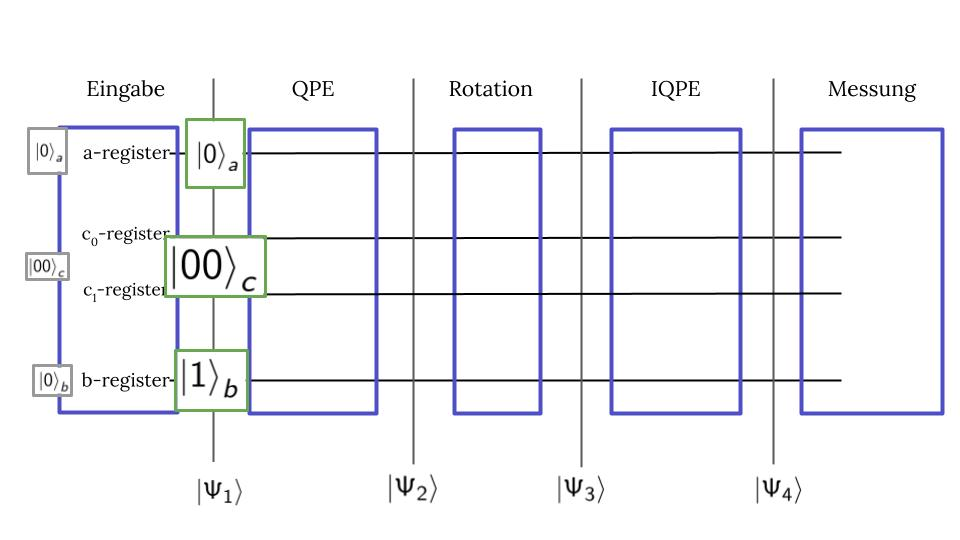
\includegraphics[width=10.5cm]{img/example_circuit/example_circuit_1.jpg}
    \end{center}

    Wir starten im 1 Zustand
    $$\ket{\Psi_1} = \ket{1}_b\ \ket{00}_c\ \ket{0}_a = \ket{1000}$$

\end{frame}


\begin{frame}
    \frametitle{Quantum Phase Estimation}
    \begin{center}
    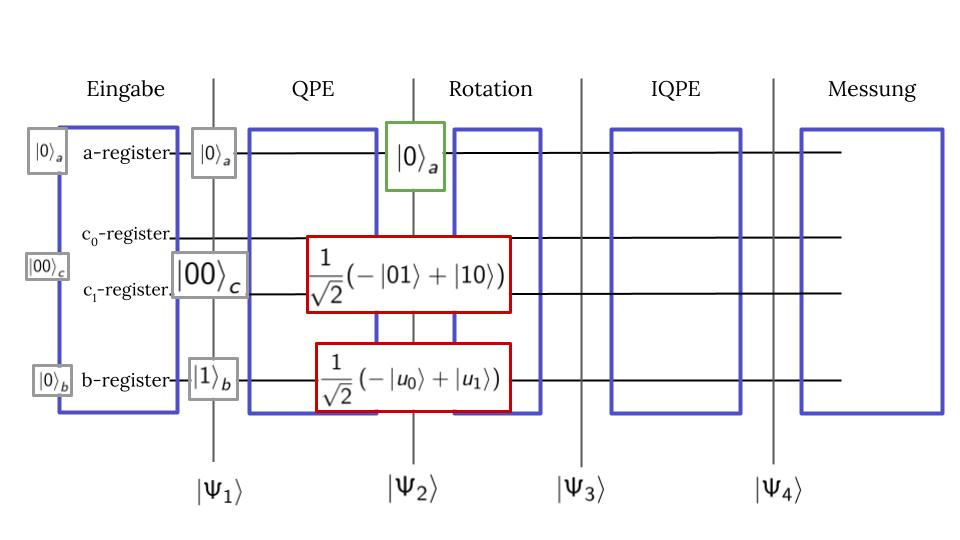
\includegraphics[width=10.5cm]{img/example_circuit/example_circuit_2.jpg}
    \end{center}

    Wir erhalten:
    $$\ket{\Psi_2} = \ket{b}_b \ket{\widetilde{\lambda}}_c\ket{0}_a$$
    $$\ket{\Psi_2} =\left(-\frac{1}{\sqrt{2}} \ket{u_0} \ket{01} +\frac{1}{\sqrt{2}}  
    \ket{u_1} \ket{10} \right)  \ket{0}_a$$

\end{frame}

\begin{frame}
    \frametitle{Ancilla Roation - Eigenwerte invertieren}
    Wir invertieren das Ancilla Qubit:
    $$ \ket{\Psi_3} = \sum_{j=0}^{2^{1}-1} b_j \ket{u_j} \ket{\widetilde{\lambda}_j} \left(\sqrt{1-\frac{C^2}{\widetilde{\lambda}_j^2}}\ket{0} + \frac{C}{\widetilde{\lambda}_j} \ket{1}\right)$$
    %$$=-\frac{1}{\sqrt{2}} \ket{u_0} \ket{01}\left(\sqrt{1-\frac{1}{1^2}}\ket{0} + \frac{1}{1} \ket{1}\right) +\frac{1}{\sqrt{2}}  \ket{u_1} \ket{10} \left(\sqrt{1-\frac{1}{2^2}}\ket{0} + \frac{1}{2} \ket{1}\right)$$
    %$$=\left(-\frac{1}{\sqrt{2}} \ket{u_0} \ket{01}\left(\ket{0} +\ket{1}\right)+\frac{1}{\sqrt{2}} \ket{u_1} \ket{10}\right)\left(\sqrt{1-\frac{1}{4}}\ \ket{0} + \frac{1}{2} \ket{1}\right)$$


    \hfil

    Wir gehen davon aus, dass wir $\ket{1}$ messen.
    $$  \ket{\Psi_3} =\sqrt{\frac{8}{5}}\left(-\frac{1}{\sqrt{2}} \ket{u_0}_b\ket{01}_c +\frac{1}{2\sqrt{2}} \ket{u_1}_b\ket{10}_c\right)\ket{1}_a $$
\end{frame}

\begin{frame}
    \frametitle{Ancilla Roation - Eigenwerte invertieren}
    \begin{center}

    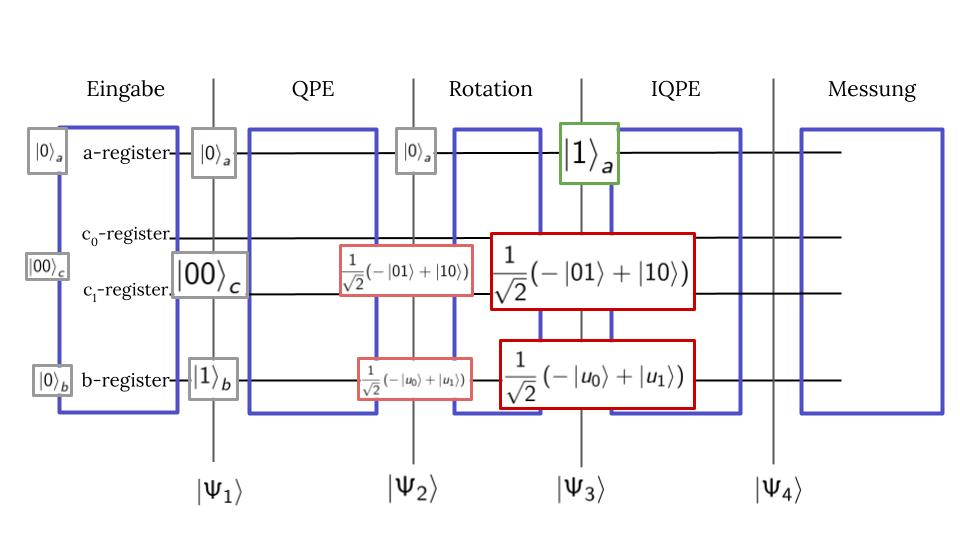
\includegraphics[width=10.5cm]{img/example_circuit/example_circuit_3.jpg}
    \end{center}
    $$ \ket{\Psi_3} =\sqrt{\frac{8}{5}}\left(-\frac{1}{\sqrt{2}} \ket{u_0}\ket{01}\ket{1} +\frac{1}{2\sqrt{2}} \ket{u_1} \ket{10}\right)\ket{1}_a$$
\end{frame}

\begin{frame}
    \frametitle{Inverse Quantum Phase Estimation}
    \begin{center}
    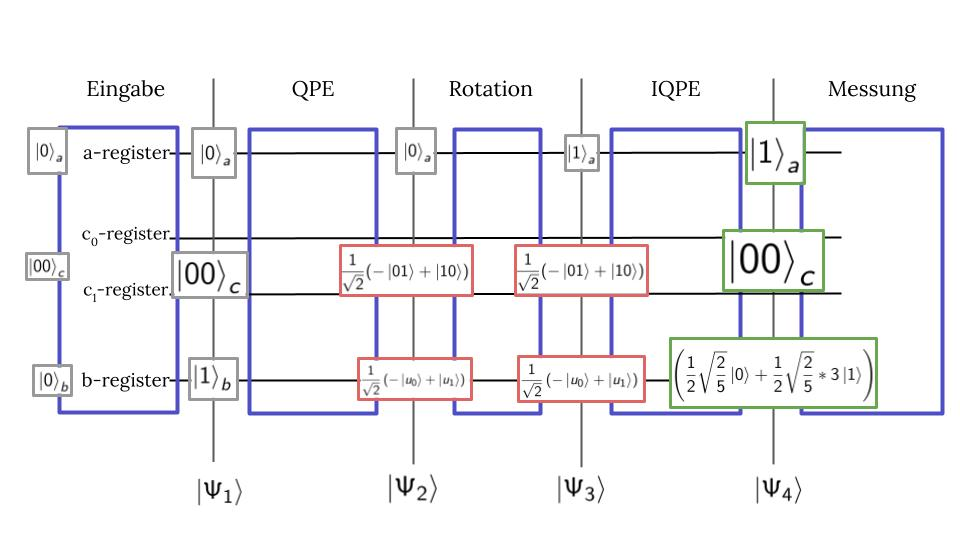
\includegraphics[width=10.5cm]{img/example_circuit/example_circuit_4.jpg}
    \end{center}

Wir erhalten:
$$\ket{\Psi_4}= \ket{x}_b \ket{00}_c \ket{1}_a $$
$$ \ket{\Psi_4}=\frac{1}{2}\sqrt{\frac{2}{5}}  \left(\ket{0} +3 \ket{1} \right) \ket{00}_b \ket{1}_a$$
\end{frame}


\begin{frame}
    \frametitle{Measurment}

Um die Wahrscheinlichkeit von $ \ket{u_0}$ und $\ket{u_1}$ zu erhalten, müssen wir ihre Koeffizienten quadrieren

$$ c_0=\left|\frac{1}{2}\sqrt{\frac{2}{5}}*1\right|^2 = \frac{1}{20} $$

$$ c_1=\left|\frac{1}{2}\sqrt{\frac{2}{5}}*3\right|^2 = \frac{9}{20} $$

Das Verhältnis im b-Register ist wie erwartet $1:9$.

\end{frame}







%\section{Evaluierung}

%\subsubsection{Laufzeit}
\begin{frame}
    \frametitle{Laufzeit}

    \textbf{Gauß Verfahren}

    $$ \mathcal{O}( N^3 ) $$

    \begin{itemize}
        \item nicht der schnellste Algorithmus
        \item gleiche constraints sind zu beachten!! 
    \end{itemize}

\end{frame}


%\subsubsection{Laufzeit}
\begin{frame}
    \frametitle{Laufzeit}
    \begin{columns}[c]


        \begin{column}{0.5\hsize}
            \textbf{Klassisch}

            Conjugate gradient descent 

            $$ \mathcal{O}(\kappa s log{\left(\frac 1 \epsilon\right)} N ) $$

            $$ \Rightarrow \mathcal{O} (N) $$

            \hfil

\onslide<3>{
            \begin{itemize}
            \item $N :=$ Anzahl an unbekannten 
            \item $\kappa= \frac {\lambda_{max}} {\lambda_{min}}$:  condition number
            \end{itemize}
}
        \end{column}
        

        \begin{column}{0.5\hsize}
            \textbf{Quanten Version}

            HHL

\onslide<2,3>{
            $$ \mathcal{O}(\frac{\kappa^2s^2}{\epsilon}logN) $$
            $$ \Rightarrow \mathcal{O} (log(N)) $$
}
            \hfil

\onslide<3>{
            \begin{itemize}
            \item $\epsilon$ := Fehler des Ergebnisses
            \item $s$ := s-sparse Matrix: jede Zeile hat max. s Einträge
            \end{itemize}
}
        \end{column}
    \end{columns}
 
    \hfil



\end{frame}


\begin{frame}
    \frametitle{Laufzeit}
    \begin{columns}[c]
        \begin{column}{0.5\hsize}
            \textbf{Klassisch}

            \hfil

            Conjugate gradient descent 

            $$ \mathcal{O}(\kappa s log{\left(\frac 1 \epsilon\right)} N ) $$

            $$ \Rightarrow \mathcal{O} (N) $$

        \end{column}
        

        \begin{column}{0.5\hsize}
            \textbf{Quanten Version}

            \hfil

            HHL

            $$ \mathcal{O}(\frac{\kappa^2s^2}{\epsilon}logN) $$

            $$ \Rightarrow \mathcal{O} (log(N)) $$
        \end{column}

    \end{columns}
 
    \hfil

    \hfil


\onslide<2>{
    \textbf{Takeaway}
    \begin{itemize}
        \item exponentialer speed up $\mathcal{O} (N)$ vs $\mathcal{O} (log(N))$
        \item klassischer algorithmus hat bessere Fehlerabhängigkeit: \\$log(\frac1{\epsilon})$ vs $\frac{1}{\epsilon}$
    \end{itemize}
}

\end{frame}



%\subsubsection{Einschränkungen}
\begin{frame}
    \frametitle{Einschränkungen}
    \begin{enumerate}[<+->]
        \item niedrige condition number $\kappa$ 

        \hfil


        \item $A$ muss s-sparse sein

        \hfil

        \item nicht jeder Eintrag von $\ket{x}$ auslesbar

        \hfil

        \item einfache Zustandsvorbereitung des Vektors $\vec b$ zum Quantenzustand $\ket{b}$

        \hfil

        \item Der Ressourcenbedarf ist hoch
\end{enumerate} \end{frame}
\section{Zukunftsperspektiven/Anwendungen}

%\subsubsection{Anwendungen}
\begin{frame}
    \frametitle{Anwendungen}

    Hauptproblem
    \begin{itemize}
        \item Hauptproblem: gibt keinen vollständigen Vektor aus
        \item Aber einige Probleme können mit dieser Methode gelöst werden:
    \end{itemize}
    
\end{frame}

\begin{frame}
    \frametitle{Anwendungen}


    Machine Learning: Least-Square-Fitting
    \begin{itemize}
        \item Datenanpassung mit Least Square Fitting
        \item durch Berechnung einer Schätzung der inversen Matrix
    \end{itemize}

   \hfil


\onslide<2>{
    Simulationen von großen Systemen 
    \begin{itemize}
        \item Elektrizitätsnetz vielen verbundenen Komponenten 
        \item geringe Anzahl Verbindungen zwischen den Komponenten
        \item Berechnung des Widerstands durch approximation von Erwartungswerten
    \end{itemize} 

   \hfil
   
}

\end{frame}

\begin{frame}
    \frametitle{Anwendung in IT-Security}


    HHL in der IT-Security
    \begin{itemize}
        \item in erster Linie nur für Lösen von linearen Systemen
        \item nicht direkt mit IT-Security verbunden
        \item aber Potenzial als Subroutine angewendet zu werden
    \end{itemize}

    \hfil

\onslide<2,3>{
    Mögliche Anwendungen
     \begin{itemize}
        \item secure multi-party computation 
        \item zero-knowledge proofs
        \item cryptographic key generation and management
        \item big data analysis/pattern recognition (für Betrugserkennung)

    \end{itemize}

\onslide<3>{
    Es wäre wichtig, mehr Anwendungen zu finden, welche den Anforderungen entsprechen. 
}

}

\end{frame}

%\subsubsection{Variationen}
\begin{frame}
    \frametitle{Optimierungen}

    Modifikationen und Optimierung
    \begin{itemize}[<+->]
        \item QRAM zur Vorbereitung von $\ket{b}$
        \item kein Ancilla-Bit erforderlich unter bestimmten Voraussetzungen 
        \item Variable time amplitude amplification um condition number $\kappa$ zu verbessern
    \end{itemize}
    
\end{frame}

%\subsubsection{Perspektive}
\begin{frame}
    \frametitle{Perspektive}

    \begin{itemize}[<+->]
        \item  Großer Einfluss im Bereich Quantum Machine Learning 
        \item  noch keine bahnbrechenden Anwendungen (wie z.B. Shors Algorithmus zum Brechen von RSA)
        \item  aber viel aktive Forschung um neue Verbesserungen im Algorithmus zu finden
        \item  zeigt deutlichen Fortschritt in der Quantencomputing Welt
    \end{itemize}
    
\end{frame}


    \begin{frame}
    \frametitle{Was das}

        \textbf{Ablauf}
        \begin{enumerate}
            \item State Preparation
            \begin{itemize}
                \item Enkodiere Vektor und Matrix in Quanten Computer
            \end{itemize}
            \item Quantum Phase Estimation
            \begin{itemize}
                \item ermittle Eigenwerte und Eigenvektoren 
                \item bilde $\ket{b}$ in Eigenbasis $A$ ab
            \end{itemize}
 
            \item Ancilla Bit Rotation - Invertieren der Eigenwerte
            \item Inverse Quantum Phase Estimation
            \item Messung

        \end{enumerate}
 
    

    \end{frame}


\end{document}